\documentclass{article}
\usepackage[letterpaper, portrait, left=25mm, right=25mm, top=25mm, bottom=25mm]{geometry}
\usepackage{parskip}
\usepackage{graphicx}
\pagenumbering{gobble}
\begin{document}

\begin{center}
\Large \sc Reference Material -- Unit 3

\bigskip

\large

\bf Note: \it You may {\em not} bring this reference to the exam on Tuesday. This is only for your practice exam,
in case you've not made your own yet. However, I will give you the moments-of-inertia information here on Tuesday
whenever you need it.
\end{center}



\vspace{2in}

Hooke's law for elasticity: $F_{\rm elastic} = -k \Delta x$

The work-energy theorem: 

$$\frac{1}{2}mv_i^2 + W_{\rm all} = \frac{1}{2}mv_f^2$$

The work-energy theorem, using potential energy:

$$\frac{1}{2}mv_i^2 + {\rm PE_i} + W_{\rm other} = \frac{1}{2}mv_f^2 + {\rm PE_f}$$

Kinetic energy of translation: $\frac{1}{2}mv^2$
Kinetic energy of rotation: $\frac{1}{2}I\omega^2$ \\

Gravitational potential energy: $mgy$ \\
Elastic potential energy: $\frac{1}{2}k(\Delta x)^2$, where $\Delta x$ is the amount by which the spring is stretched or compressed

\bigskip

If an object rotates at angular velocity $\omega$, a point at radius $r$ moves at a speed $v_T = \omega r$.

\newpage

\begin{center}
\begin{tabular}{l | l}

 \multicolumn{1}{c|}{\Large Translation} & \multicolumn{1}{c}{\Large Rotation} \\
 \\
\hline
\hline
 & \\
Position $\vec s$ & Angle $\theta$ \\
Velocity $\vec v$ & Angular velocity $\omega$ \\
Acceleration $\vec a$ & Angular acceleration $\alpha$ \\
 & \\
\hline
\hline
 & \\
Kinematics: $\vec s(t)\frac{1}{2}\vec at^2 + \vec v_0 t + \vec s_0$ & $\theta(t) = \frac{1}{2}\alpha t^2 + \omega_0 t + \theta_0$ \\
 & \\
\hline
\hline

 & \\
Force $\vec F$ & Torque $\tau$ \\
Mass $m$ & Rotational inertia $I$ \\
Newton's second law $\vec F = m \vec a$ & Newton's second law for rotation $\tau = I \alpha$ \\
 & \\

\hline
\hline

 & \\
Kinetic energy $KE=\frac{1}{2}mv^2$ & Kinetic energy $KE=\frac{1}{2}I\omega^2$ \\
Work $W = \vec F \cdot \Delta \vec s$ & Work $W = \tau \Delta \theta$ \\
Power $P = \vec F \cdot \vec v$ & Power $P = \tau \omega$ \\
 & \\

\hline
\hline

 & \\
Momentum $\vec p = m \vec v$ & Angular momentum $L = I\omega$ (extended object)\\
& \hspace{8.7em} $L = mvr_\perp$ (point-like object) \\
 & \\

\hline
\end{tabular}

\bigskip

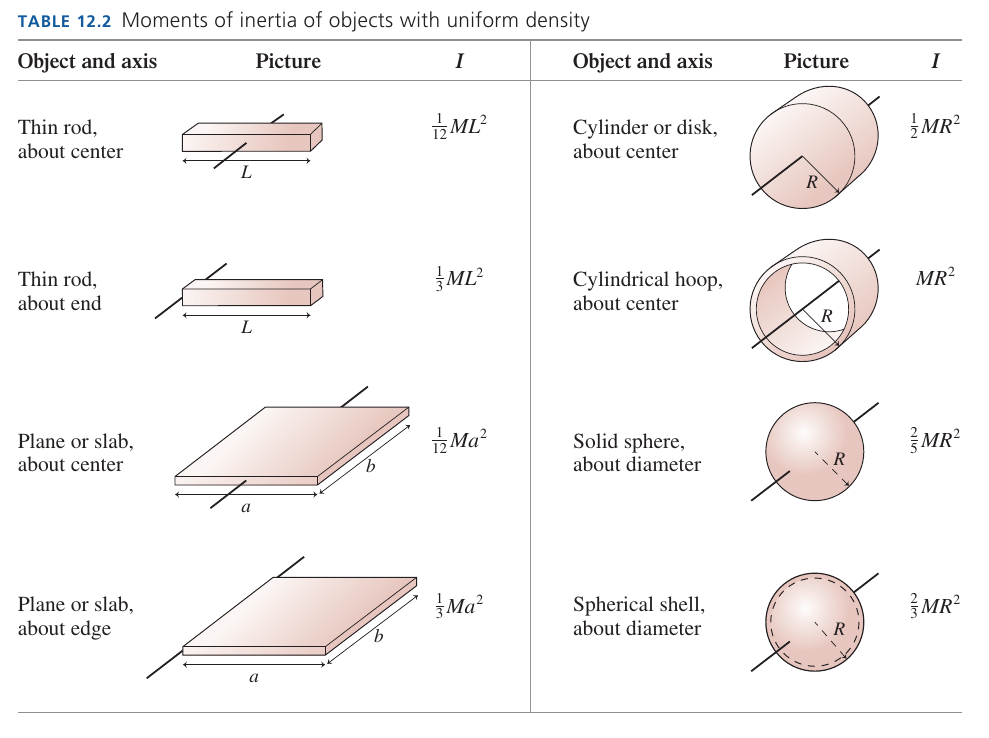
\includegraphics[width=0.7\textwidth]{moment-table.png}

\end{center}



\end{document}
